\section{Vergleich Beurer BM55 und Omnitest 3}
Biosignal BM55: Blutdruck \\
Biosignal Omnitest 3: Glukosegehalt im Blut \\
\begin{figure}[h!]
    \centering
    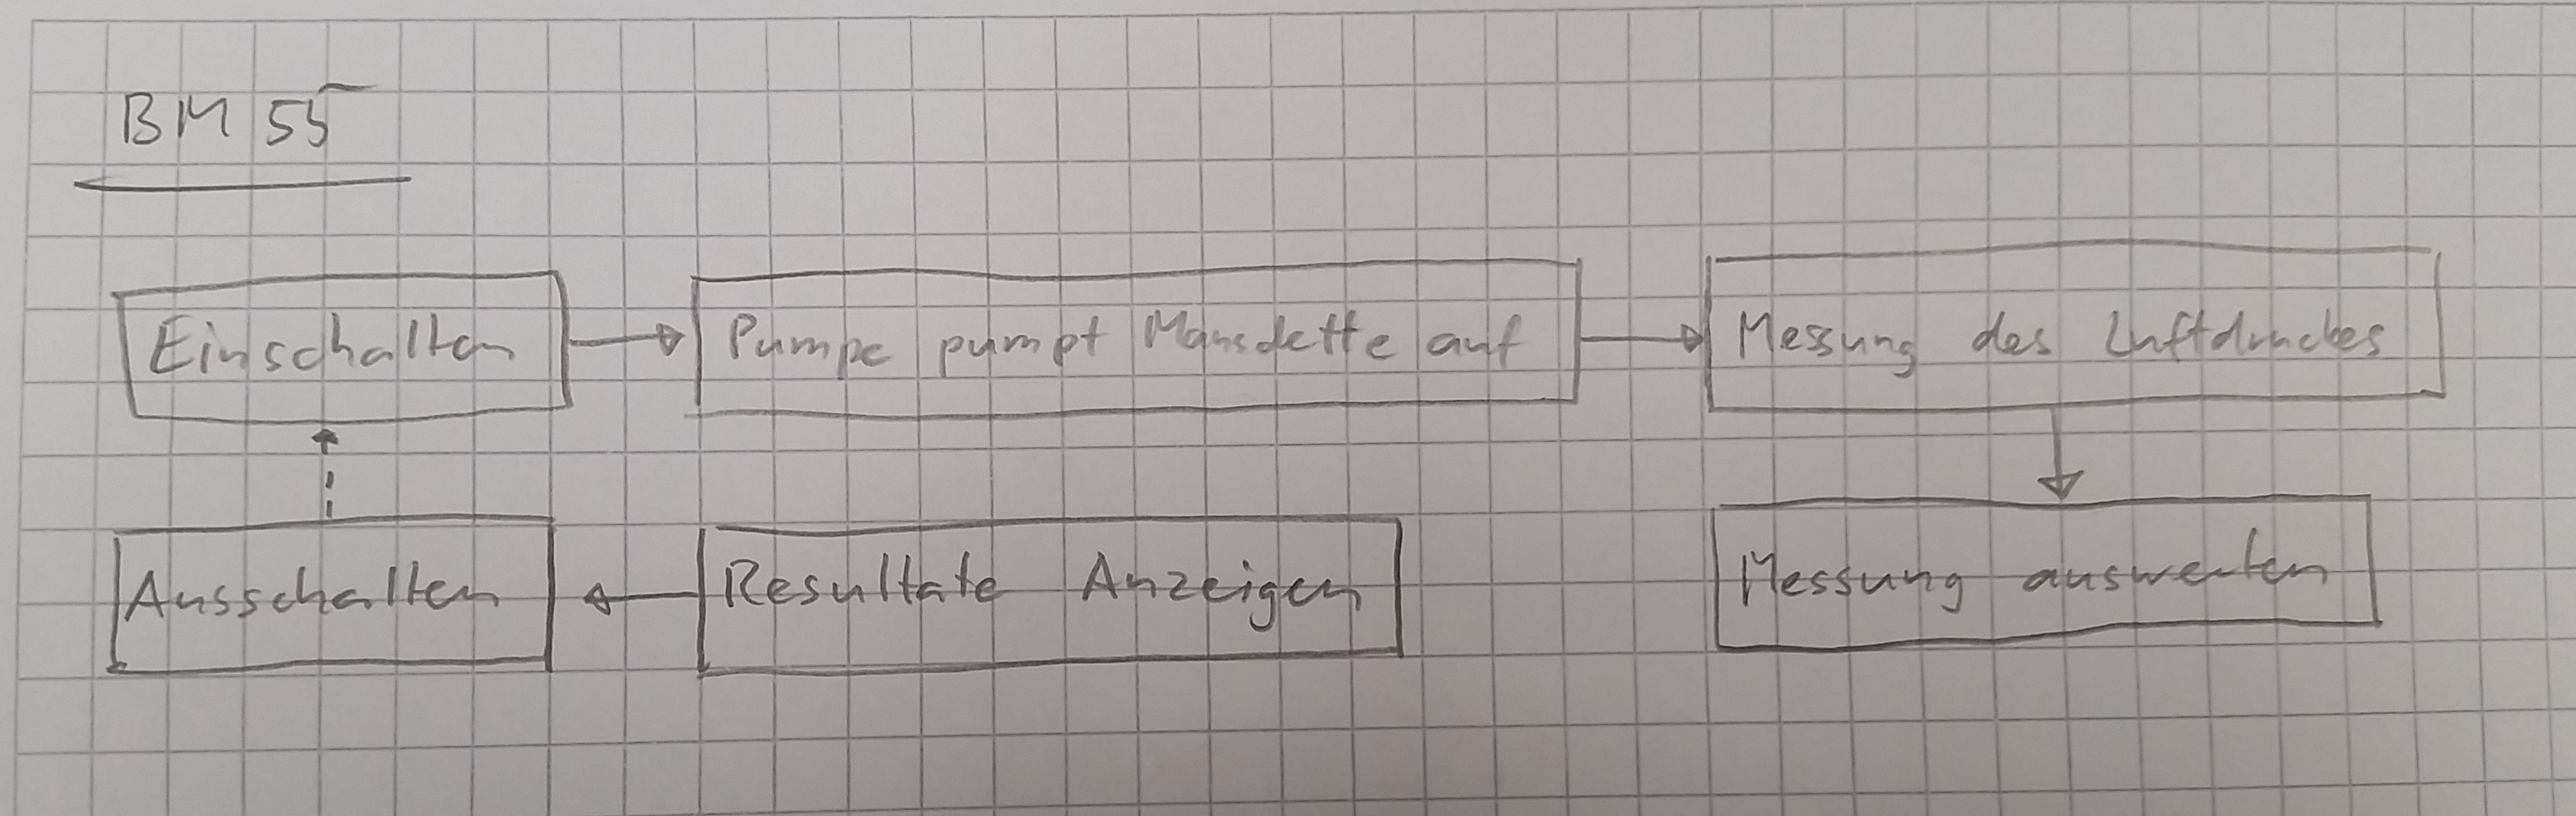
\includegraphics[width=0.7\textwidth]{Ablauf_BM55.jpg}
    \caption{Blockschaltbild BM55}
\end{figure}
\begin{figure}[h!]
    \centering
    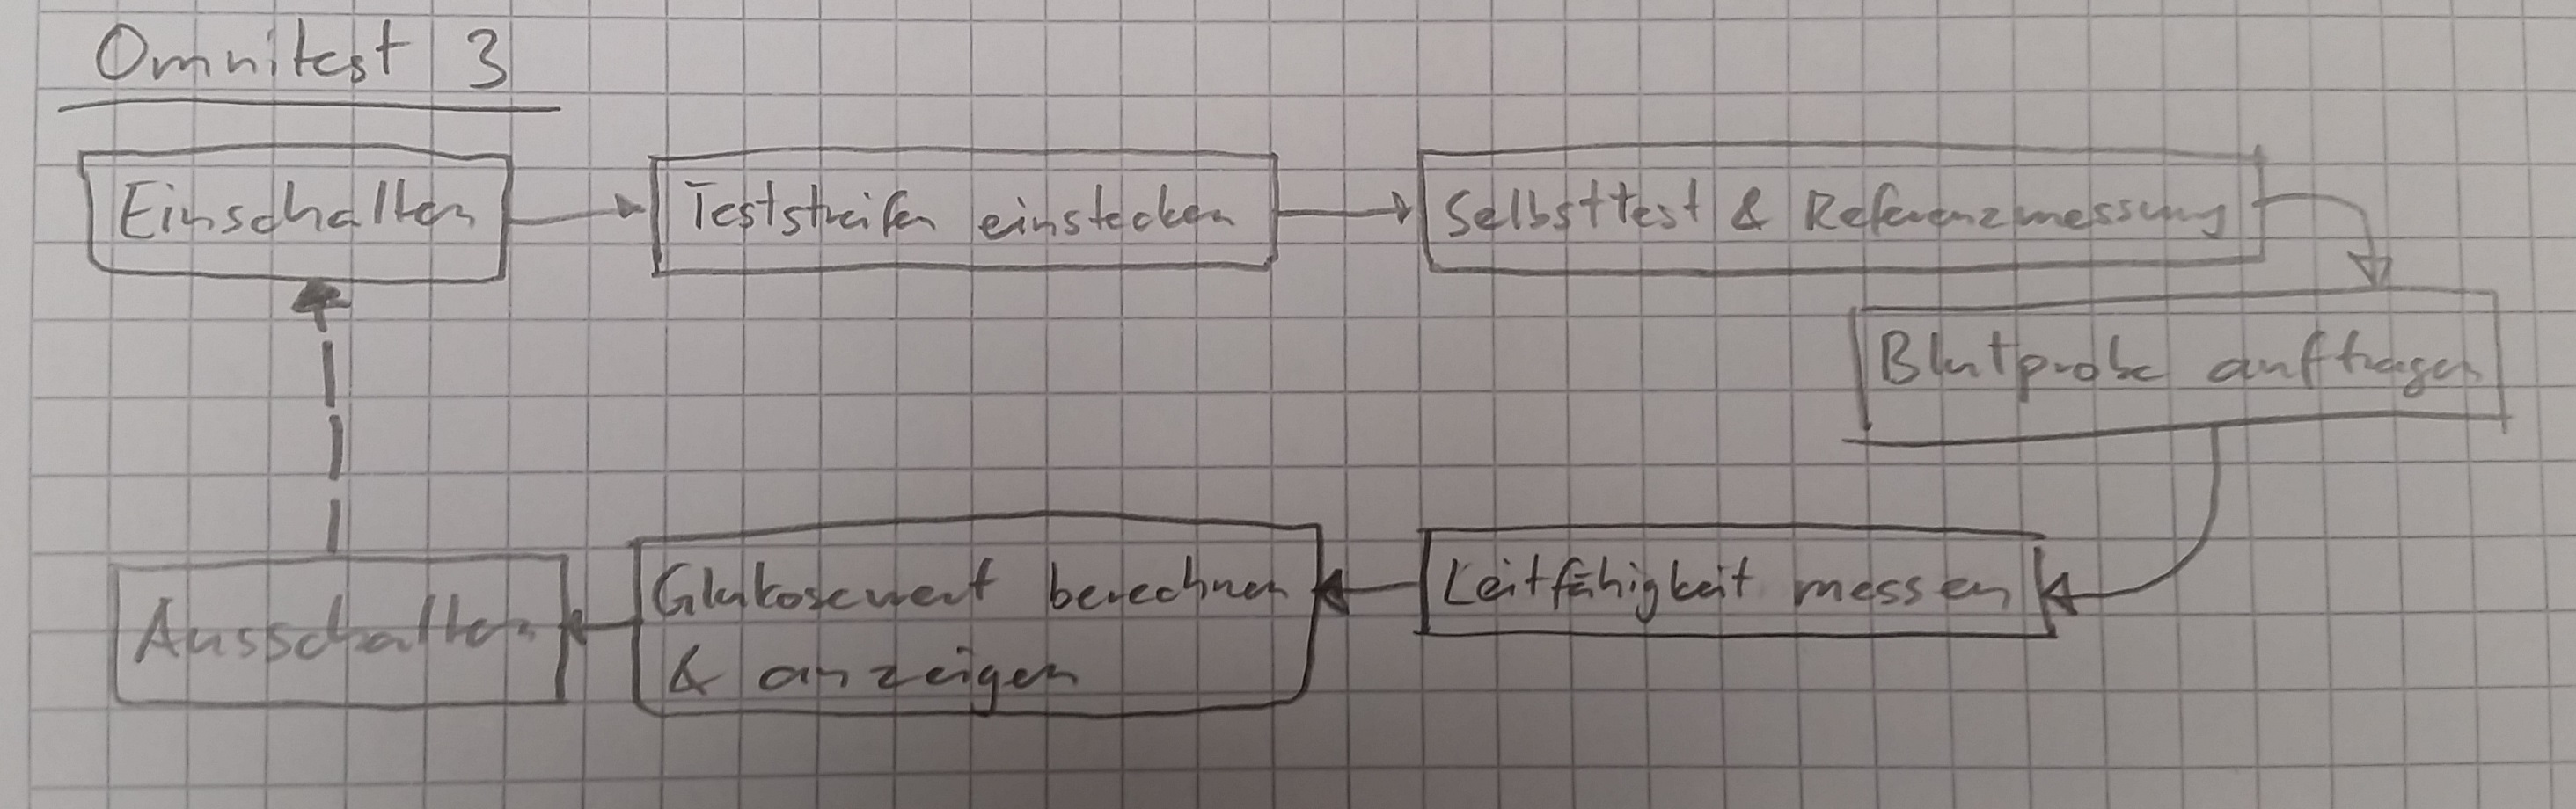
\includegraphics[width=0.7\textwidth]{Ablauf_Omnitest_3.jpg}
    \caption{Blockschaltbild Omnitest 3}
\end{figure}
Trägermedium BM55: Luftdruck \\
Trägermedium Omnitest 3: Elektrische Leitfähigkeit \\
Vorteile BM55: 
\begin{itemize}
    \item Einfache Anwendung
\end{itemize}
Nachteile BM55: 
\begin{itemize}
    \item Eingeschränkte Genauigkeit
    \item Störfaktoren
\end{itemize}
Vorteile Omnitest 3: 
\begin{itemize}
    \item Direkte Messung auf Trägermedium
\end{itemize}
Nachteile Omnitest 3: 
\begin{itemize}
    \item Infektionsgefahr
    \item Umständliche Messung
    \item Biogefährdender Abfall
\end{itemize}
